
\documentclass{package/notes}
\usepackage[english]{babel}
\usepackage{amssymb,amsmath,amsfonts}  %%% for maths
%%%%%%%%%%%%%%%%%%%%%%%%%%%%%%%%%%%%%
\usepackage{package/color-env}
\usepackage{lipsum}
\usepackage{tikz}
\renewcommand\qedsymbol{$\blacksquare$}
%%%%%%%%%%%%%%%%%%%%%%%%%%%%%%%%%%%%%

\begin{document}

	\begin{titlepage} % Suppresses headers and footers on the title page
		
		\centering % Centre everything on the title page
		
		\scshape % Use small caps for all text on the title page
		
		\vspace*{\baselineskip} % White space at the top of the page
		
		%------------------------------------------------
		%	Title
		%------------------------------------------------
		
		\rule{\textwidth}{1.6pt}\vspace*{-\baselineskip}\vspace*{2pt} % Thick horizontal rule
		\rule{\textwidth}{0.4pt} % Thin horizontal rule
		
		\vspace{0.75\baselineskip} % Whitespace above the title
		
		{\huge AP PHYSICS 1 NOTES\\} % Title
		
		\vspace{0.75\baselineskip} % Whitespace below the title
		
		\rule{\textwidth}{0.4pt}\vspace*{-\baselineskip}\vspace{3.2pt} % Thin horizontal rule
		\rule{\textwidth}{1.6pt} % Thick horizontal rule
		
		\vspace{2\baselineskip} % Whitespace after the title block
		
		%------------------------------------------------
		%	Subtitle
		%------------------------------------------------
		
		\LARGE{Notes for any AP Physics 1 Course or Algebra-Based University Physics Course} 
		
		\vspace*{3\baselineskip} % Whitespace under the subtitle
		
		
		
		\vspace{0.5\baselineskip} 
		
		
		
		\vspace{0.5\baselineskip} 
		
		
		
		\vfill 
		
		%------------------------------------------------
		% Author
		%------------------------------------------------
		
		
		\vspace{0.3\baselineskip} 
		
		
		{\large Edited by\\  Trevor Bushnell} 
		
	\end{titlepage}
	\tableofcontents
%\newpage
\chapter*{Introduction}

This document aims to highlight the important content of the AP Physics 1 course in traditional notes format. These notes are completely open-source, which means anyone is allowed to use these notes for their own personal benefit without having to seek permission from myself. \newline

While these notes are designed for an AP Physics 1 course, all of the content seen in the AP Physics 1 Course and Exam Description document written by College Board will be included within these notes. However, this does \textit{not} mean that the content will be covered in the same way or order that is laid out in the Course and Exam Description. Additionally, the AP Physics 1 course is designed to be equivalent to a one-semester algebra-based physiscs course at a university level, meaning that the content that is covered within these notes is just as applicable for any one-semester agebra-based physics course at the university level. \newline

Due to the open-source nature of these notes, anyone is allowed to contribute to improving these notes as they see fit. Since I am using \LaTeX to write these notes and I am using GitHub to distribute these notes easily, you must request all changes through the repository website on GitHub, which you can find \textbf{here}. If you are interested in contributing to these notes, then there are a few ways that you can do so:\newline

\begin{enumerate}
	\item \textbf{Open and submit an issue on my GitHub repository:} I write all my notes in \LaTeX, which is a typesetting language that is really helpful when it comes to typing and rendering math equations quickly and easily. If you do not know how to write \LaTeX code but are still interested in making a change to the notes, you can open an issue by going to the MathNotes repo on GitHub, and clicking on the button labeled "New Issue." From there, you can type out the change that you wish to see in the notes. It would be helpful if you would indicate what course you would like to see changed so that I can understand what you are referring to. I will then update the code to include your issue so that you don't have to worry about writing the code yourself.
	\item \textbf{Create and submit a pull request:} If you know how to write LaTeX code and you understand how GitHub works, you can submit a pull request where you can write the code that you want to change yourself. I will then review the code and either submit the code to be incorporated into the notes OR provide some comments on your code if I wish for something to be different. 
\end{enumerate}

Thank you so much for using these notes. I hope that the information is provided in such a way that it can help you when reviewing content for you AP test/class exam and just in general when it comes to learning the content for the course. Happy studying!



\chapter{Kinematics}

This unit talks about motion, both in 1D and 2D. Motion analysis has a scientific name called kinematics. The goal of kinematics is to be able to describe where an object is in relation to a starting position, how fast the object is moving, and how much the object's speed is changing. 

\section{Definition of Terms}

\begin{itemize}
	\item \textbf{POSITION} ($x$): The location that you are at wrt the origin (starting place/point/position)
	\begin{itemize}
		\item position is a \textit{scalar}
		\item SI Units: meters (m)
	\end{itemize}
	\item \textbf{DISPLACEMENT} ($\Delta x$): Change in position
	\begin{itemize}
		\item how far you go from an initial starting position (you can start at the origin or another position)
		\item displacement is a \textit{vector} (has direction and magnitude)
		\item SI Units: meters
		\begin{definition}[Formulas for Displacemnt]{def:label}
			$$\Delta x = x_f - x_i$$
			In English: An object's displacement ($\Delta x$) is equal to an object's final position ($x_f$) minus an object's initial position ($x_i$) 
		\end{definition}
	\end{itemize}
	\item \textbf{VELOCITY} ($v$): An object's change in position (displacement) over a certain period of time
	\begin{itemize}
		\item How fast you are going in a given direction
		\item velocity is a \textit{vector} (it has a direction and magnitude)
		\item SI Units: $\frac{m}{s}$ (meters per second)\newpage
		\begin{definition}[Formulas for Velocity]{def:label}
			$$v = \frac{\Delta x}{\Delta t}$$
			In English: Velocity ($v$) is equal to displaecment ($\Delta x$) divided by the total change in time ($\Delta t$)
			$$v = v_f - v_i$$
			In English: An object's velocity ($v$) is equal to an object's final velocity ($v_f$) minus an object's initial velocity ($v_i$) 
		\end{definition}
	\end{itemize}
	\item \textbf{SPEED} ($S$): How fast you are going (does \textbf{not} account for which direction you are going)
	\begin{itemize}
		\item scalar (only has \textit{magnitude} and not direction)
		\item SI Units: $\frac{m}{s}$ (meters/second)
		\item to calculate an object's speed, simply find the magnitude of the object's velocity
	\end{itemize}
	\item \textbf{ACCELERATION} ($a$): Change in velocity with respect to time
	\begin{itemize}
		\item How fast it takes something to speed up/slow down
		\item acceleration is a \textit{vector} (has both direction and magnitude)
		\item SI Units: $\frac{m}{s^2}$ (meters per second per second OR meters per second-squared)
		\begin{definition}[Formulas for Acceleration]{def:label}
			$$a = \frac{\Delta v}{\Delta t}$$
			In English: Acceleration ($a$) is equal to an object's change in velocity ($\Delta V$) divided by the total change in time ($\Delta t$)
			$$a = a_f - a_i$$
			In English: An object's acceleration ($a$) is equal to an object's final acceleration ($a_f$) minus an object's initial acceleration ($a_i$) 
		\end{definition}
	\end{itemize}
\end{itemize}


\subsection{A Quick Note on Frames of Reference}

\begin{itemize}
	\item a \textbf{frame of reference} is simply your perspective on a given physical situation
	\item your frame of reference will determine what you perceive to be positive/negative directions and might change certain orientations
	\item EXAMPLE: viewing motion left and right versus viewing motion in front/behind you would cause the direction of displacement, velocity, and acceleration to be forward/backward instead of left/right
\end{itemize}\newpage

\section{Graphical Analysis of Motion}

There are many different types of motion graphs that one can encounter. All graphs and their relative important information is summarized in the following subsections.

\subsection{Position VS Time Graphs}

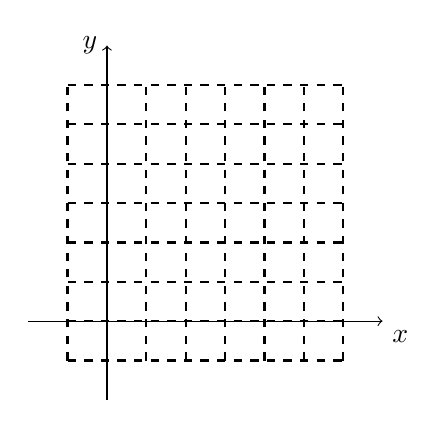
\begin{tikzpicture}[domain=0:2] % COME BACK AND INCLUDE AN EXAMPLE OF A POSITION VS TIME GRAPH

	\draw[thick,color=black,step=.5cm,dashed] (-0.5,-.5) grid (3,3);
	\draw[->](-1,0) -- (3.5,0)
	node[below right] {$x$};
	\draw[->] (0,-1) -- (0,3.5)
	node[left] {$y$};
\end{tikzpicture}

\begin{itemize}
	\item \textbf{y-axis:} position ($x$)
	\item \textbf{x-axis:} time ($t$)
	\item \textbf{slope of the graph:} velocity ($v$)
	\begin{itemize}
		\item the steeper the slope, the faster the object moves
		\item if the slope is like a front slash (/), then the object has positive velocity
		\item if the slope is like a backslash (\textbackslash), then the object has negative velocity
	\end{itemize}
\end{itemize}


\subsection{Velocity VS Time Graphs}

% INSERT A FIGURE OF A VELOCITY VS TIME GRAPH HERE

\begin{itemize}
	\item \textbf{y-axis:} velocity ($v$)
	\item \textbf{x-axis:} time ($t$)
	\item \textbf{slope of the graph:} acceleration ($v$)
	\begin{itemize}
		\item the steeper the slope, the faster the object accelerates
		\item if the slope is like a front slash (/), then the object has positive acceleration
		\item if the slope is like a backslash (\textbackslash), then the object has negative acceleration
	\end{itemize}
\end{itemize}




\end{document}
.